\begin{figure}
  \setlength{\unitlength}{\textwidth}

  \begin{picture}(1,0.72)
%(0,0.35)
    
    % % %Parkinson Data 
    \put(0.025,0.48){\includegraphics[width=0.5\unitlength]{../FnP/gnuplot/displacement_amp_re_parkinson_1.eps}}
    \put(0.025,0.25){\includegraphics[width=0.5\unitlength]{../FnP/gnuplot/velocity_amp_re_parkinson.eps}}
    \put(0.025,0.02){\includegraphics[width=0.5\unitlength]{../FnP/gnuplot/mean_power_re_parkinson.eps}}
    
    % Re 165 Data 
    \put(0.495,0.48){\includegraphics[width=0.5\unitlength]{../FnP/gnuplot/displacement_amp_re165.eps}}
    \put(0.495,0.25){\includegraphics[width=0.5\unitlength]{../FnP/gnuplot/velocity_amp_re165.eps}}
    \put(0.495,0.02){\includegraphics[width=0.5\unitlength]{../FnP/gnuplot/mean_power_re_165.eps}}
   
%    \put(0.25,0.93){\ustar}
%    \put(0.8,0.93){\ustar}
%    \put(0.25,0.63){\ustar}
%   \put(0.8,0.63){\ustar}
    \put(0.25,0.0){\ustar}
    \put(0.75,0.0){\ustar}
    
    \put(0.00,0.6){$\displaystyle\frac{A}{D}$}
%    \put(0.52,1.075){$\frac{A}{D}$}
    \put(0.00,0.4){$\displaystyle\frac{V}{D}$}
%    \put(0.52,0.83){$\frac{V}{D}$}
    \put(-0.025,0.15){$\displaystyle\frac{P_{m}}{\rho \mathcal{A}U^3 }$}
%    \put(0.5,0.54){$\frac{P_{m}}{\rho \mathcal{A}U^3 }$}
    
    \put(0.085,0.685){\small(a)}
    \put(0.555,0.685){\small(b)}
    \put(0.085,0.455){\small(c)}
    \put(0.555,0.455){\small(d)}
    \put(0.085,0.225){\small(e)}
    \put(0.555,0.225){\small(f)}   
  \end{picture}

%  \vspace{-4cm}
  \caption{Velocity amplitude, displacement amplitude and mean power  as functions of $U^*$. Data presented in (a), (c) and (e) were calculated using input data at $Re=22300$ and $m^*=1163$ obtained by \cite{Parkinson1964} at three different damping ratios: $\zeta=0.0125$ (\ding{83}), $\zeta=0.015$ (\ding{116}) and $\zeta=0.0175$ (\ding{108}). Data presented in (b),(d) and (f) were obtained using input data at $Re=165$ and $m^*=20$ at three different damping ratios: $\zeta=0.075$ ($\times$), $\zeta=0.1$ (\ding{117}) and $\zeta=0.15$ (+). The multiple branches for the higher Re are due to the hysteresis between two solutions.}
  
\label{fig:uncollapsed_data}
\end{figure}


